% !TEX program = xelatex

\documentclass[hidelinks, 12pt, a4paper]{article}

\usepackage{fontspec}
\setmainfont[Ligatures=TeX]{Linux Libertine O}

\usepackage[hidelinks, colorlinks = true, urlcolor = blue]{hyperref}

\usepackage{indentfirst}
\usepackage{graphicx}
\usepackage{subcaption}
\usepackage[left=2cm,right=2cm,top=2cm,bottom=2cm]{geometry}
\usepackage{lipsum}

\graphicspath{{../logs/session2}{../media/session2}}


\begin{document}

\begin{titlepage}

\begin{figure}[h!]
  \begin{center}
    
\includegraphics[width=3cm]{assets/auth.pdf}
    \label{fig:cover_auth_logo}
  \end{center}
\end{figure}

\centering
\Large Αριστοτέλειο Πανεπιστήμιο Θεσσαλονίκης\\
\Large Πολυτεχνική Σχολή\\
%\large Τμήμα Ηλεκτρολόγων Μηχανικών και Μηχανικών Υπολογιστών\\
%\large Τομέας Τηλεπικοινωνιών

\vspace{\fill}

%\LARGE \textbf{Java socket programming} \\
\LARGE \textbf{Δίκτυα Υπολογιστών Ι}

\vspace{\fill}

\Large Θεόδωρος Κατζάλης \\
\Large ΑΕΜ:9282 \\ 
\Large katzalis@auth.gr

\vspace{\fill}
\raggedright

\centering
\vspace{\fill}
\today

\end{titlepage}

%\maketitle


\pagebreak
{
\renewcommand*\contentsname{Περιεχόμενα}
\hypersetup{linkcolor=black}
\tableofcontents
}
\pagebreak

% \section{Lorem}
% \lipsum

\section{Settings}

Οι ρυθμίσεις του virtual modem ήταν οι ακόλουθες:
\[speed = 80.000 \quad (bps)\]

\section{G1}

\begin{figure}[h!]
\centering
	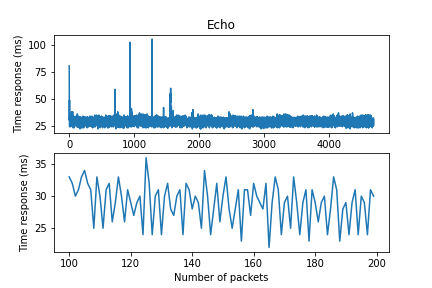
\includegraphics[keepaspectratio, width=.7\textwidth]{echo.png}
	\caption{15/04/2021 14:59:51 "E6777"} 
\end{figure}

\begin{figure}[h!]
\centering
	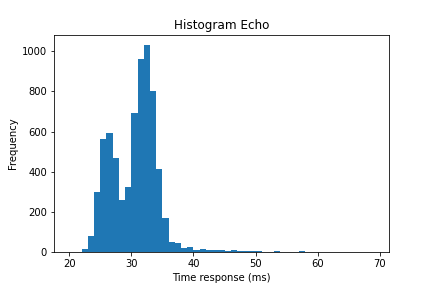
\includegraphics[keepaspectratio, width=.7\textwidth]{hist_echo.png}
	\caption{Ιστόγραμμα echo packets \\ 15/04/2021 14:59:51 "E6777"} 
\end{figure}

\pagebreak

\section{G2}

\begin{figure}[h!]
\centering
	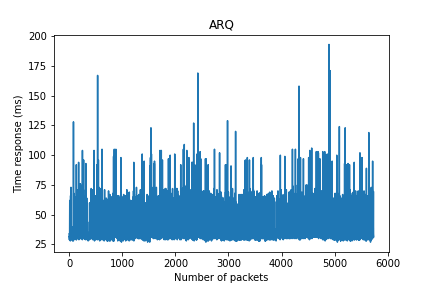
\includegraphics[keepaspectratio, width=.8\textwidth]{arq.png}
	\caption{15/04/2021 14:59:51 ACK: "Q4219" NACK: "R9877"} 
\end{figure}


\section{G3}

\begin{figure}[h!]
\centering
	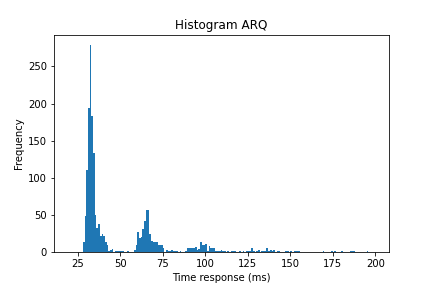
\includegraphics[keepaspectratio, width=.8\textwidth]{hist_arq.png}
	\caption{15/04/2021 14:59:51 ACK: "Q4219" NACK: "R9877"} 
\end{figure}

\pagebreak

\section{E1}

\begin{figure}[h!]
     \begin{subfigure}[b]{0.5\textwidth}
         \centering
         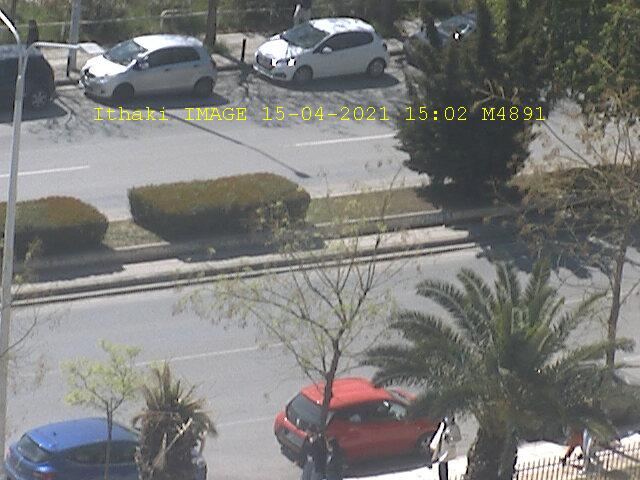
\includegraphics[keepaspectratio, width=\textwidth]{image_error_free_fix.jpg}
         \caption{CAM=FIX \\ 15/04/2021 14:59:51 "M4891"}
     \end{subfigure}
     \begin{subfigure}[b]{0.5\textwidth}
         \centering
         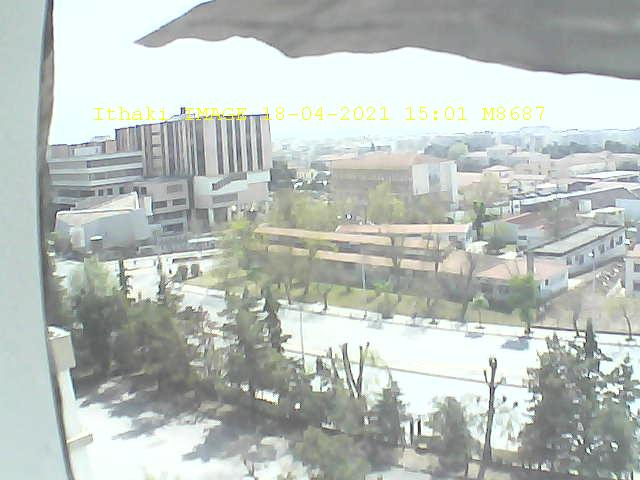
\includegraphics[keepaspectratio, width=\textwidth]{image_error_free_ptz.jpg}
         \caption{CAM=PTZ \\ 15/04/2021 14:59:51 "M4891"}
     \end{subfigure}
     \caption{Εικόνες δίχως θόρυβο}
\end{figure}


\section{E2}

\begin{figure}[h!]
     \begin{subfigure}[b]{0.5\textwidth}
         \centering
         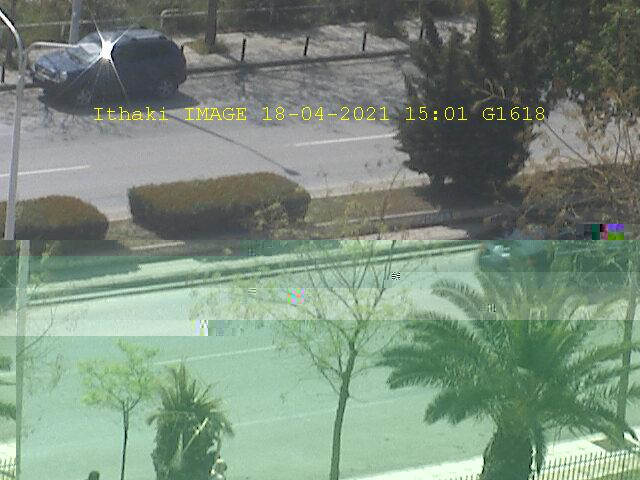
\includegraphics[keepaspectratio, width=\textwidth]{image_with_errors_fix.jpg}
         \caption{CAM=FIX \\ 15/04/2021 14:59:51 "G1562"}
     \end{subfigure}
     \hfill
     \begin{subfigure}[b]{0.5\textwidth}
         \centering
         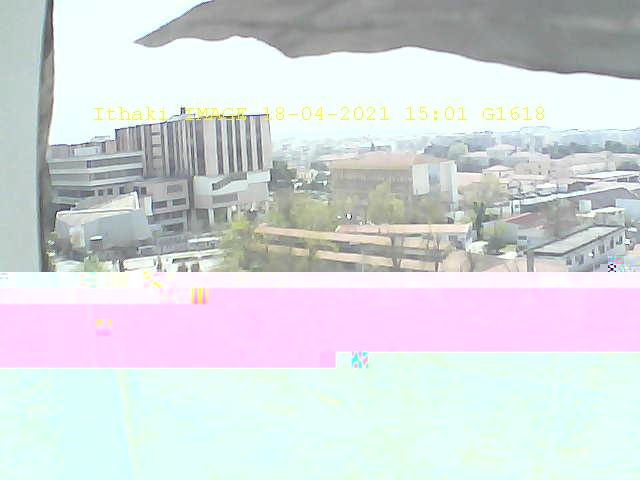
\includegraphics[keepaspectratio, width=\textwidth]{image_with_errors_ptz.jpg}
         \caption{CAM=PTZ \\ 15/04/2021 14:59:51 "G1562"}
     \end{subfigure}
     \caption{Εικόνες με θόρυβο}
\end{figure}

\pagebreak

\section{M1}

\begin{figure}[h!]
\centering
	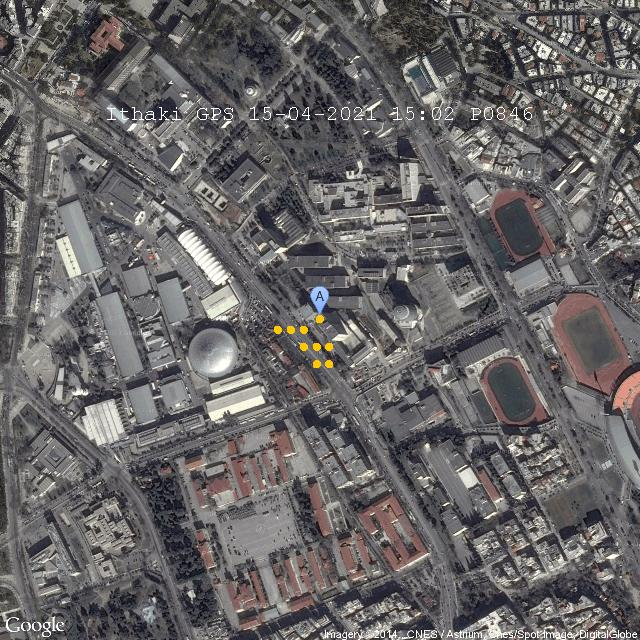
\includegraphics[keepaspectratio, width=.8\textwidth]{gps.jpg}
    \caption{15/04/2021 14:59:51 "P0846" \\ "P0846R=1000099"} 
\end{figure}


\section{Bit error rate}

\[BER:0.0011577804153436455\]

\end{document}
